\subsubsection{GPU Footprint and Utilization}
\label{subsec:gpu-usage}

Figure \ref{fig:gpu-usage} shows the GPU memory footprint and processing core utilization for each scenario.
For \texttt{sionnart}, allocated memory is almost flat.
It is $337$ MiB for the smallest stationary scenario, about $465$-$469$ MiB for most scenarios, and $491$ MiB for the largest high-mobility scenario.
This is because most of the memory usage is due to the Sionna RT scene and increasing number of stations in the same scene, not the number of packets processed by ns-3.
By contrast, \texttt{ns3sionna} grows significantly in the high-mobility scenario.
The memory increases from $730$ MiB at $N=1$ to $7858$ MiB at $N=32$.

\begin{figure}[t]
    \centering
    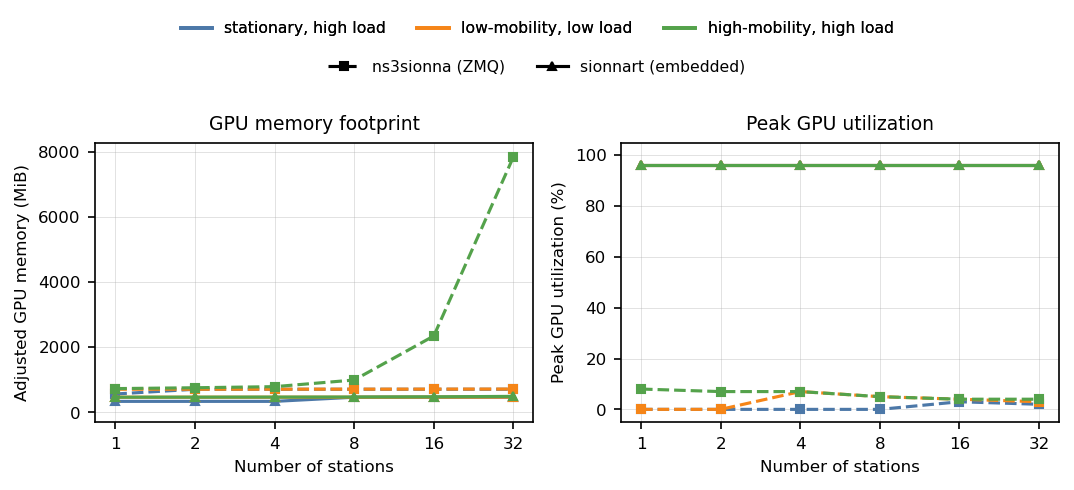
\includegraphics[width=\linewidth]{images/gpu_usage.png}
    \caption{Reported GPU memory footprint and peak utilization for the two
        Sionna-backed backends.}
    \label{fig:gpu-usage}
\end{figure}

The peak-utilization panel present the maximum observed value but not the average GPU load.
\texttt{sionnart} utilize upto $96\%$ at its peak for performing the channel calculations but the duration of running at peak is very short.
On the other hand, \texttt{ns3sionna} has lower peak utilization but the GPU is busy most of the time.

In summary, \texttt{sionnart} keeps a nearly fixed GPU memory footprint because the scene and others are reused across channel queries.
\texttt{ns3sionna} uses much more memory because it has to keep per-link ray-tracing state as the number of mobile links increases.
For \texttt{sionnart}, it utilize full potential of GPU and duration of running calculation is very short while the \texttt{ns3sionna} is busy most of the time with lower peak utilization.